% ----------------------------------------------------------------------------
% INLETS E OUTLETS
% ----------------------------------------------------------------------------

\chapter{Inlets e outlets}

Os objetos que criamos até agora são inúteis.
Não servem para nada, pois não se comunicam com outros objetos nem modificam
sinais de áudio.
Para dar utilidade a um \external, é necessário que ele comunique com outros objetos
do Pure Data.
Isto é feito por meio de \emph{inlets} e \emph{outlets}, portas
de entrada e saída (respectivamente) de sinais de áudio e/ou mensagens.

Neste capítulo vamos tratar exclusivamente de inlets e outlets de mensagens.
Entre os inlets de mensagem há os tipos passivos e ativos, que os usuários
costumam chamar de inlets frios e quentes.
Inlets \textbf{passivos} são inlets cujo valor recebido é associada diretamente
a um atributo do objeto.
São chamados de passivos pois a alteração do seu valor não resulta na chamada
de um método e a atribuição do valor recebido ao atributo do objeto é feita
automaticamente.
Inlets \textbf{ativos}, por outro lado, são associados a
funções e permitem a execução de uma função arbitrária quando um valor é
recebido no inlet.

As mensagens passadas para o objeto em seus inlets ocorre por passagem de valor
para o caso de inteiros e por passagem de parâmetros para os demais tipos.
Por isto, é necessário cuidado ao manipular tais mensagens pois a alteração do
valor de um ponteiro implica na alteração do mesmo em todos os objetos que o
recebe.
Veja o exemplo \texttt{inverter.c}.
Neste exemplo o valor de um Symbol é alterado e resulta no mesmo invertido.
Caso você inverta este valor, salve o patch, feche-o e abra-o novamente, encontrará o
valor deste símbolo invertido, conforme apresentado nas Figuras \ref{fig:inverter} e
\ref{fig:inverter2}.

\begin{figure}[h!]
\centering
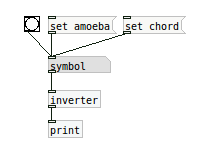
\includegraphics[scale=\Mysize]{inverter}
\caption{Alteração de uma mensagem recebida.}
\label{fig:inverter}
\end{figure}

\begin{figure}[h!]
\centering
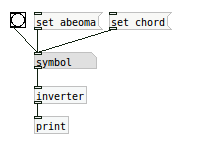
\includegraphics[scale=\Mysize]{inverter2}
\caption{Alteração de uma mensagem recebida, ao reabrir.}
\label{fig:inverter2}
\end{figure}


% -----+-----+-----+-----+-----+-----+-----+-----+-----+-----+-----+-----+-----+
%      |     |     |     |     |     |     |     |     |     |     |     |     |
% -----+-----+-----+-----+-----+-----+-----+-----+-----+-----+-----+-----+-----+
\section{Inlets ativos}

Um inlet ativo sempre recebe mensagens no primeiro inlet do objeto e por isto
o mesmo deve ser utilizado com a classe do tipo \texttt{CLASS\_DEFAULT}.
Estes inlets são sempre associados a uma função.
A criação de um inlet ativo define o tipo do átomo que o inlet receberá (veja o
exemplo 05 e o resultado na figura \ref{fig:inlet-ativo}).

\begin{lstlisting}[caption=Exemplo de objeto com inlet ativo]
// all inlet-methods receive the object as their first argument.
void example5_bang(t_example5 *x) { 
  post("BANGED!");
}

void example5_anything(t_example5 *x, t_symbol *s, int argc, t_atom *argv){
  post("ANYTHING!");
}

void example5_setup(void) {
  example5_class = class_new(gensym("example5"),
    (t_newmethod) example5_new, // Constructor
    0, 
    sizeof (t_example5),
    CLASS_DEFAULT,
    0); // LAST argument is ALWAYS zero
  class_addbang(example5_class, example5_bang);
  class_addanything(example5_class, example5_anything);
}
\end{lstlisting}

Neste exemplo, definimos duas funções associadas ao primeiro inlet, uma para
receber uma mensagem \texttt{bang} e outra para receber qualquer tipo de dado.
O resultado desta implementação pode ser vista na Figura \ref{fig:inlet-ativo}.

\begin{figure}[h!]
\centering
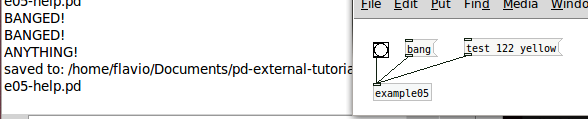
\includegraphics[scale=\Mysize]{example5}
\caption{Inlets ativos.}
\label{fig:inlet-ativo}
\end{figure}

Abaixo, a tabela com os métodos que criam inlets ativos,
e assinaturas possíveis para funções associadas a cada tipo:

\begin{center}
\begin{tabular}{|l|l|}
\hline
método do pd para criar inlet ativo & assinatura para o método associado ao
inlet \\
\hline
\texttt{class\_addbang(t\_class *c, t\_method fn);}   & \texttt{my\_b(t\_myt *x);} \\
\texttt{class\_addfloat(t\_class *c, t\_method fn);}  & \texttt{my\_f(t\_myt *x, t\_floatarg f);} \\
\texttt{class\_addsymbol(t\_class *c, t\_method fn);} & \texttt{my\_s(t\_myt *x,t\_symbol *s);} \\
\texttt{class\_addpointer(t\_class *c, t\_method fn);}& \texttt{my\_p(t\_myt *x, t\_gpointer *pt);} \\
\texttt{class\_addlist(t\_class *c, t\_method fn);}   & \texttt{my\_l(t\_myt *x, t\_symbol *s, int argc, t\_atom *argv);} \\
\texttt{class\_addanything(t\_class *c, t\_method fn);}& \texttt{my\_a(t\_mydata *x, t\_symbol *s, int argc, t\_atom *argv);} \\
\hline
\end{tabular}
\end{center}

% -----+-----+-----+-----+-----+-----+-----+-----+-----+-----+-----+-----+-----+
%      |     |     |     |     |     |     |     |     |     |     |     |     |
% -----+-----+-----+-----+-----+-----+-----+-----+-----+-----+-----+-----+-----+
\section{Mensagens para o primeiro inlet}

Da mesma maneira que é possível mapear os tipos de dados recebidos no primeiro
inlet para funções, também é possível definir tipos de mensagens separadamente.
Isto é feito através da função \texttt{add\_method()} (veja o exemplo 08).
Esta função permite que a mensagem possua um identificador com seu tipo e outros
dados que acompanham esta mensagem.

\begin{lstlisting}[caption=Passagem de mensagens para o primeiro inlet]
// Constructor of the class
void * example8_new(void) {
  t_example8 *x = (t_example8 *) pd_new(example8_class);
  return (void *) x;
}

void example8_start(t_example8 *x){
  post("START / BANG");
}

void example8_open(t_example8 *x, t_symbol *s){
  post("open %s",s->s_name);
}


void example8_alfa(t_example8 *x, t_floatarg f){
  post("ALFA VALUE %f",f);
}

void example8_setup(void) {
  example8_class = class_new(gensym("example8"),
    (t_newmethod) example8_new, // Constructor
    (t_method) example8_destroy, // Destructor
    sizeof (t_example8),
    CLASS_DEFAULT,
    0); // LAST argument is ALWAYS zero
  // All these messages will be received by the first left inlet
  class_addmethod(example8_class, (t_method) example8_start, 
    gensym("start"), 0); // two messages, the same function
  class_addmethod(example8_class, (t_method) example8_start, 
    gensym("bang"),  0); // may be "start" or "bang" messages
  class_addmethod(example8_class, (t_method) example8_open,  
    gensym("open"),  A_DEFSYMBOL,0);
  class_addmethod(example8_class, (t_method) example8_alfa,  
    gensym("alfa"), A_DEFFLOAT,0); 
}
\end{lstlisting}

A listagem acima mostra que as mensagens \texttt{bang} e \texttt{start} são
associadas ao mesmo método.
Além disto, a mensagem \texttt{open} recebe um texto como parâmetro e a mensagem
\texttt{alfa} recebe um float como parâmetro.
Como no construtor, a função \texttt{class\_addmethod} pode receber uma lista de
e receber um valor zero como último argumento.

Desta forma não precisamos tratar a mensagem que o inlet recebe mas definí-las
de antemão e criar funções que mapeiem a mensagem recebida.
Veja a Figura \ref{fig:mais-inlets}.

\begin{figure}[h!]
\centering
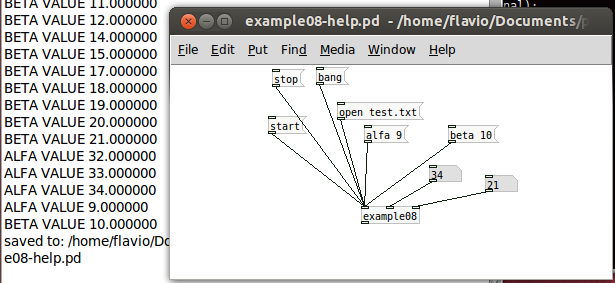
\includegraphics[scale=\Mysize]{example8}
\caption{Mais inlets.}
\label{fig:mais-inlets}
\end{figure}

% -----+-----+-----+-----+-----+-----+-----+-----+-----+-----+-----+-----+-----+
%      |     |     |     |     |     |     |     |     |     |     |     |     |
% -----+-----+-----+-----+-----+-----+-----+-----+-----+-----+-----+-----+-----+
\section{Inlets passivos}

Um inlet passivo é a forma de o objeto receber uma mensagem que não está
associado a uma função mas a um atributo do objeto.
Assim, ao criarmos um inlet que recebe um valor float, o mesmo deverá alterar um
atributo float do objeto sem que o mesmo possua uma função associada para
verificar esta alteração.
Por não possuir uma função associada, tal inlet é comumente chamado de ``inlet
frio''.
Abaixo vemos um exemplo de objeto com um inlet passivo (veja a figura
\ref{fig:inlet-passivo}):

\begin{lstlisting}[caption=Exemplo de inlet passivo]
static t_class *example4_class;

typedef struct _example4 {
  t_object x_obj;
  t_float my_float;
} t_example4;

// Constructor of the class
void * example4_new(t_symbol * arg1, t_floatarg arg2) {
  t_example4 *x = (t_example4 *) pd_new(example4_class);
  floatinlet_new(&x->x_obj, &x->my_float);
  return (void *) x;
}
\end{lstlisting}

Neste exemplo, o atributo \texttt{my\_float} do objeto é associado a um inlet do
tipo float.
Isto  significa que, caso tenhamos uma mensagem float ligada a este objeto, o valor
desta mensagem ficará armazenada no atributo my\_float.

Um inlet passivo é associado a um tipo do Pure Data, e requer que o atributo
associado seja do mesmo tipo do valor recebido através do inlet.
Para cada tipo do Pure Data, utiliza-se uma função diferente para criar inlets
que recebam aquele tipo (veja o exemplo evenodd.c).

As funções para criar os inlets passivos são:

\begin{itemize}
\item \texttt{floatinlet\_new(t\_object *owner, t\_float *fp)}
\item \texttt{symbolinlet\_new(t\_object *owner, t\_symbol **sp)}
\item \texttt{pointerinlet\_new(t\_object *owner, t\_gpointer *gp)}
\end{itemize}

Para adicionar inlets passivos de um tipo genérico, veja a Subseção Proxy de inlets
adiante.

\begin{figure}[h!]
\centering
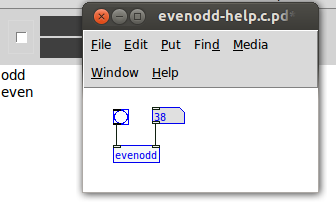
\includegraphics[scale=\Mysize]{evenodd}
\caption{Inlet passivo (do arquivo exemplo evenodd.c)}
\label{fig:inlet-passivo}
\end{figure}


% -----+-----+-----+-----+-----+-----+-----+-----+-----+-----+-----+-----+-----+
%      |     |     |     |     |     |     |     |     |     |     |     |     |
% -----+-----+-----+-----+-----+-----+-----+-----+-----+-----+-----+-----+-----+
\section{Um inlet ativo extra}

A função \texttt{inlet\_new()} pode adicionar novos inlets a um objeto sem que 
estes inlets sejam passivos.
Tal função depende de haver uma mensagem associada ao primeiro inlet e utiliza
a função presente nesta associação para receber os dados deste inlet.
Por esta razão, apesar de o mesmo parecer um inlet passivo,
este novo inlet não é associado a um atributo mas a uma função associada a
símbolos de mensagens:

\begin{lstlisting}[caption=Criando inlets ativos extras]
t_inlet *inlet_new(t_object *owner, t_pd *dest,
      t_symbol *s1, t_symbol *s2);
\end{lstlisting}

Neste caso, quando um átomo do tipo \texttt{s1} for recebido neste inlet, o
mesmo será passado para a função associada a mensagem \texttt{s2}.
Veja o exemplo abaixo.

\begin{lstlisting}

// Constructor of the class
void * example08_new(void) {
   t_example08 *x = (t_example08 *) pd_new(example08_class);
   // creates inlets for distinct messages
   inlet_new(&x->x_obj, &x->x_obj.ob_pd, gensym("float"), gensym("alfa"));
   inlet_new(&x->x_obj, &x->x_obj.ob_pd, gensym("float"), gensym("beta"));
   (...)
}

void example08_setup(void) {
  example08_class = class_new(gensym("example08"),
    (t_newmethod) example08_new, // Constructor
   ...
  // associate messages with inlets 2 and 3
  class_addmethod(example08_class, (t_method) example08_alfa, gensym("alfa"), A_DEFFLOAT,0); 
  class_addmethod(example08_class, (t_method) example08_beta, gensym("beta"), A_DEFFLOAT,0); 
}
\end{lstlisting}

Neste exemplo, criamos um método para aceitar as mensagens \texttt{alfa} e \texttt{beta}.
Se estas mensagens forem recebidas pelo inlet quente, suas funções serão chamadas
para tratar a mensagem.
Além disto, dois inlets passivos foram criados para receber dados do tipo float
e tais inlets foram associados às mensagens \texttt{alfa} e \texttt{beta}.
Por esta razão este inlet não é tão passivo assim.
O método para processar a mensagem alfa será chamado tanto se esta
mensagem for enviada quanto se um valor float for passaro para o segundo inlet,
como mostrado na figura \ref{fig:example8}.

\begin{figure}[h!]
\centering
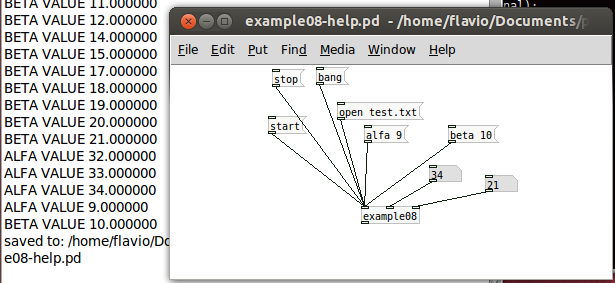
\includegraphics[scale=\Mysize]{example8}
\caption{Inlets criado pela função inlet\_new}
\label{fig:example8}
\end{figure}

% -----+-----+-----+-----+-----+-----+-----+-----+-----+-----+-----+-----+-----+
%      |     |     |     |     |     |     |     |     |     |     |     |     |
% -----+-----+-----+-----+-----+-----+-----+-----+-----+-----+-----+-----+-----+
\section{Proxy de inlets}
Com os inlets apresentados até agora é impossível criar um objeto que possua
um inlet passivo que aceite qualquer tipo de mensagem pois o PD não possui um
método para isto.
Tal implementação só é possível utilizando um proxy de inlet.
Esta técnica pode ser vista no exemplo ``yourclass.c''\footnote{Exemplo adaptado do
site:\url{http://puredata.info/Members/mjmogo/proxy-example-for-pd.zip/at_download/file}.

Este exemplo possui modificações feitas pelos autores deste tutorial.}.

A ideia básica deste \external é definir não um mas dois objetos sendo primeiro
utilizado para suas funcionalidades e o outro utilizado apenas para ser o
proxy.

\begin{lstlisting}[caption=Estruturas de dados para um proxy]
/*
 * declare the proxy object class
 */
t_class *proxy_class = NULL;

/*
 * declare your class
 */
t_class *yourclass_class = NULL;

typedef struct _proxy {
	t_pd l_pd;
	// if you want to maintain a pointer to your main class,
	// if not, besure to change the 'init' function
	void *yourclass;
} t_proxy;

typedef struct _yourclass {
	t_object x_obj;
	t_proxy pxy;
} t_yourclass;

\end{lstlisting}

A classe proxy não tem um atributo do tipo \texttt{t\_object} mas um um objeto do tipo
\texttt{t\_pd}.
A sua classe terá um atributo do tipo sua classe proxy.

O próximo passo é o método setup de sua classe chamar o método setup da classe
proxy, que contará com um inlet do tipo anything.

\begin{lstlisting}[caption=configuração de um inlet proxy]
static void proxy_setup(void) {
	post("proxy_setup");
	proxy_class =
		(t_class *)class_new(gensym("proxy"),
							 (t_newmethod)proxy_new,
							 (t_method)proxy_free,
							 sizeof(t_proxy),
							 0,
							 A_GIMME,
							 0);
	class_addanything(proxy_class, (t_method)proxy_anything);
}

void yourclass_setup(void) {
	post("yourclass_setup");
	yourclass_class =
		(t_class *)class_new(gensym("yourclass"),
							 (t_newmethod)yourclass_new,
							 (t_method)yourclass_free,
							 sizeof(t_yourclass),
							 0,
							 A_GIMME,
							 0);
	
	// be sure to call the proxy class setup before we finish
	proxy_setup();
}
\end{lstlisting}

Na criação da sua classe, o atributo \texttt{yourclass} e o atributo \texttt{l\_pd} da
classe proxy recebem atribuições.
Um inlet é criado e associado a classe proxy e seu método \texttt{proxy\_anything}.

\begin{lstlisting}[caption=Criação da classe com um inlet proxy]
static void *yourclass_new(t_symbol *s, int argc, t_atom *argv) {
   t_yourclass *x = (t_yourclass *)pd_new(yourclass_class);
   if (x) {
      // first make the sql_buffer
      x->pxy.l_pd = proxy_class;
      x->pxy.yourclass = (void *) x;
      
      // this connects up the proxy inlet
      inlet_new(&x->x_obj, &x->pxy.l_pd, 0, 0);
      post("yourclass_new");
   }
   return x;
}
\end{lstlisting}

Agora basta definir o método anything para a classe proxy e um método anything
para a sua clase.

\begin{lstlisting}[caption=Passagem de dados da classe proxy para a classe principal]
void yourclass_anything(t_yourclass *x, t_symbol *s, int argc, t_atom *argv){
   int i;
   char buf[SYMBOL_LENGTH];
   post("yourclass_anything: %s", s -> s_name);
   for(i = 0; i < argc; i++) {
      atom_string(&argv[i], buf, SYMBOL_LENGTH);
      post("argv[%d]: %s", i, buf);
   }

}

static void proxy_anything(t_proxy *x, t_symbol *s, int argc, t_atom *argv){
   post("Proxy Anything");
   yourclass_anything((t_yourclass *) x->yourclass, s, argc, argv);
}
\end{lstlisting}

Vale notar que nem sempre é necessário que a classe proxy passe os dados para a
classe que possui o inlet, podendo o tratamento da mensagem ser feito na função
do próprio inlet.

O resultado desta implementação pode ser verificado na Figura\ref{fig:proxy}.

\begin{figure}[h!]
\centering
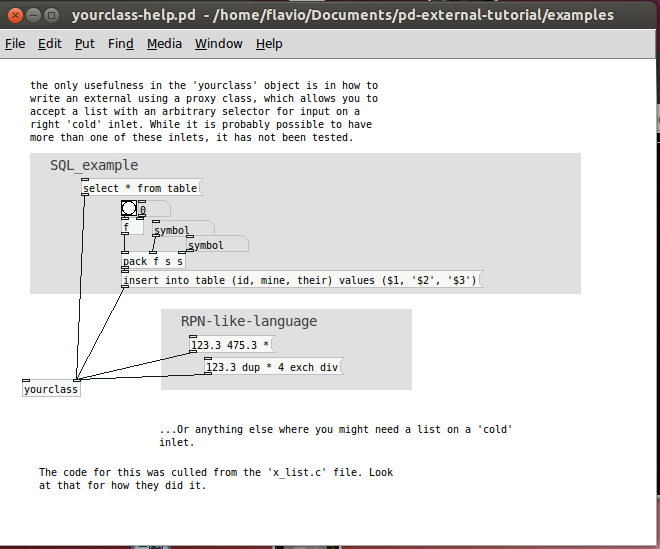
\includegraphics[scale=\Mysize]{proxy}
\caption{Proxy}
\label{fig:proxy}
\end{figure}

% -----+-----+-----+-----+-----+-----+-----+-----+-----+-----+-----+-----+-----+
%      |     |     |     |     |     |     |     |     |     |     |     |     |
% -----+-----+-----+-----+-----+-----+-----+-----+-----+-----+-----+-----+-----+
\section{Oulets}

Depois de termos tratado as formas de entrada de dados através de inlets do
Pure Data, chegou a hora de falarmos das saídas. A saída de dados dos objetos
do Pure Data é feita por meio de outlets (veja o exemplo 06).

\begin{lstlisting}[caption=Exemplo de outlet]
typedef struct _example6 {
  t_object x_obj;
  t_outlet *my_outlet; // Defines an outlet
} t_example6;

// The BANG method, first inlet
void example6_bang(t_example6 *x) {
  post("BANGED!");
  outlet_bang(x->my_outlet); // Bang my outlet
}

// Constructor of the class
void * example6_new(t_symbol * arg1, t_floatarg arg2) {
  t_example6 *x = (t_example6 *) pd_new(example6_class);
  x->my_outlet = outlet_new(&x->x_obj, gensym("bang"));
  return (void *) x;
}

void example6_setup(void) {
    example6_class = class_new(gensym("example6"),
      (t_newmethod) example6_new, // Constructor
      0, 
      sizeof (t_example6),
      CLASS_DEFAULT,
      A_DEFFLOAT, // First Constructor parameter
      A_DEFSYMBOL, // Second Consctructo parameter
      0); // LAST argument is ALWAYS zero
    class_addbang(example6_class, example6_bang);
}
\end{lstlisting}

Um outlet deve ser definido na estrutura do objeto e instanciado pela função
\texttt{outlet\_new()}, definindo também o tipo do átomo associado.
No caso deste exemplo, o outlet é do tipo \texttt{bang} e dispara um bang toda
vez que recebe um bang (veja a figura \ref{fig:outlet-bang}).

\begin{figure}[h!]
\centering
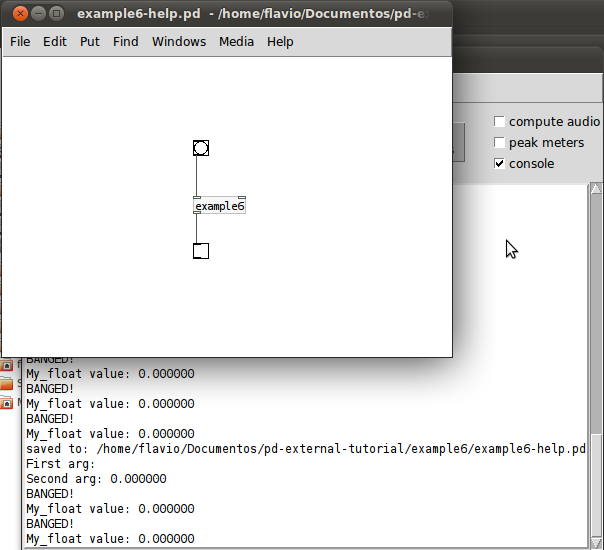
\includegraphics[scale=\Mysize]{example6}
\caption{Um external bem útil que recebe um bang e envia um bang.}
\label{fig:outlet-bang}
\end{figure}

Há funções definidas para enviar vários tipos diferentes para um outlet.
São elas:

\begin{itemize}
\item void outlet\_bang(t\_outlet *x);
\item void outlet\_pointer(t\_outlet *x, t\_gpointer *gp);
\item void outlet\_float(t\_outlet *x, t\_float f);
\item void outlet\_symbol(t\_outlet *x, t\_symbol *s);
\item void outlet\_list(t\_outlet *x, t\_symbol *s, int argc, t\_atom *argv);
\item void outlet\_anything(t\_outlet *x, t\_symbol *s, int argc, t\_atom *argv);
\end{itemize}

Vale lembrar que é de bom tom liberar a memória alocada para o outlet no destrutor
da classe.
Esta desalocação pode ser feita pela função abaixo:

\begin{lstlisting}[caption=Desalocando a memória]
   outlet_free(x->x_outlet_inverted_symbol);
\end{lstlisting}

% -----+-----+-----+-----+-----+-----+-----+-----+-----+-----+-----+-----+-----+
%      |     |     |     |     |     |     |     |     |     |     |     |     |
% -----+-----+-----+-----+-----+-----+-----+-----+-----+-----+-----+-----+-----+
\section{IOlets dinâmicos}
Alguns objetos, como o trigger, cria outlets dinamicamente conforme a quantidade
de parâmetros recebidos.
Tal abordagem pode ser utilizada tanto para inlets passivos quanto para outlets
pois a criação destes ocorre no método construtor e não no método setup da
classe.
No exemplo ``multiplus.c'', a quantidade de inlets e outlets depende de um
parâmetro passado para o construtor.
Neste caso, guardamos na estrutura do objeto uma lista de outlets e um atributo
com a quantidade de outlets.

\begin{lstlisting}[caption=Estrutura de um objeto com outlets dinâmicos]
typedef struct _multiplus {
   t_object x_obj;
   t_float count;
   t_float * values;
   t_outlet ** my_outlets; // Defines a outlet
} t_multiplus;
\end{lstlisting}

No construtor, dependendo da passagem de um parâmetro que nos diz quantos outlets
desejamos possuir, criamos e alocamos dinamicamente os outlets.

\begin{lstlisting}[caption=Criação dinâmica de inlets e outlets]
void * multiplus_new(t_floatarg count_arg){
   t_multiplus *x = (t_multiplus *) pd_new(multiplus_class);
   x->count = count_arg;
   x->my_outlets = getbytes(x->count * sizeof(t_outlet*));
   x->values = getbytes(x->count * sizeof(t_float));
   int i = 0;
   for(i = 0 ; i < (int) x->count; i++){
      x->my_outlets[i] = outlet_new(&x->x_obj, gensym("bang"));
      floatinlet_new (&x->x_obj, &x->values[i]);
   }
   return (void *) x;
\end{lstlisting}

Não esquecer de desalocar os outlets no destrutor dos objetos.

\begin{lstlisting}[caption=Destrutor com outlets dinâmicos]
void outlet_dinamico_destroy(t_outlet_dinamico *x) {
   int i = 0;
   for(i = 0 ; i < (int) x->outlet_count; i++){
     outlet_free(x->my_outlets[i]);
   }
}
\end{lstlisting}

Neste exemplo hipotético e talvez nada útil, ao receber uma mensagem de bang
o objeto irá retornar os valores recebidos em seus inlets + 1.

\begin{lstlisting}[caption=Destrutor com outlets dinâmicos]
void multiplus_bang(t_multiplus *x){
   int i = 0;
   for(; i < (int) x->count ; i++){
      outlet_float(x->my_outlets[i], x->values[i] + 1);
   }
}
\end{lstlisting}

O resultado desta implementação pode ser visto na Figura\ref{fig:multiplus}.

\begin{figure}[h!]
\centering
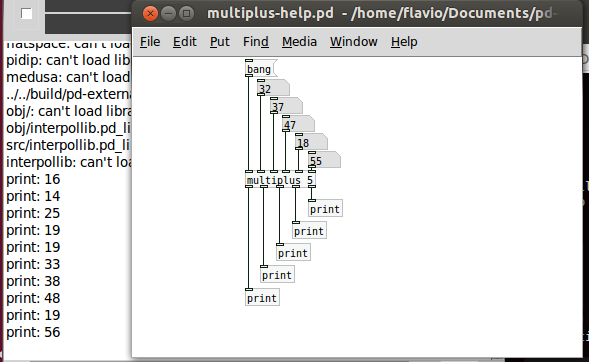
\includegraphics[scale=\Mysize]{multiplus}
\caption{Inlets e outlets criados dinamicamente.}
\label{fig:multiplus}
\end{figure}

